%!TEX root = thesis.tex
\chapter{Corner Transfer Matrix}
\label{chapter:ctm}
The \textit{cerner transfer matrix renormalization group} (CTMRG) \cite{} is an algorithm to numerically compute the \textit{effective environments} which is an approximation of the environment of systems. For example, if the infinite PEPS is composed by a single tensor $A^{h}_{uldr}$ repeatedly, where $h$ express a physical basis of  $\mathbb{V}$ with dimension $d$, and $u,l,d,r$ are virtual bonds with dimension $D$, see Fig. \ref{fig501}(a). Then we can represent the scale norm $\Braket{\psi|\psi}$ by a simple two dimensional tensor network $\varepsilon$ which is characterized by reduced tensors $a$, shown in Fig. \ref{fig501}(b). The reduced tensor $a$ is defined as eq.\ref{reduce_a}, 
\begin{align}
	\label{reduce_a}
	a \equiv \sum_{h=1}^{d} A_{h} \otimes A^{*}_{h}
\end{align}
The environment $\varepsilon^{[\vec{r}]}$ of the site $\vec{r}$ could be described by the reduced tensors in the gray rectangles in Fig.\ref{fig501}(c) and the \textit{effective environments} $G^{[\vec{r}]}$ shown in Fig. \ref{fig501}(d) is target of the CTMRG. 

In the following subsections, we will show more details of implementation of CTM and compare some features between obtaining the states from iPEPE and PESS.

\begin{figure}[ht]
	\centering
	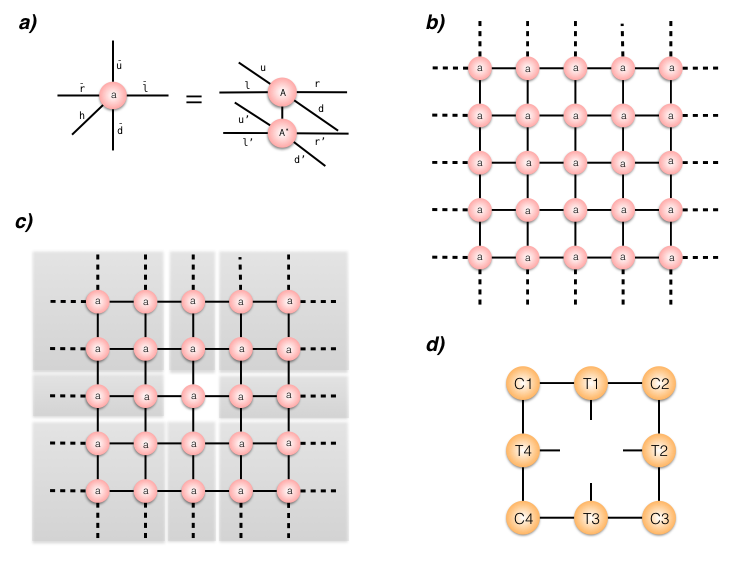
\includegraphics[width=0.75\textwidth]{figures/fig501.png}
	\caption[The picture of the main idea of itebd.]{The red and blue tensor denotes on \textit{odd} and \textit{even} sites. The yellow one are time evolution operators $e^{-\tau H_{k,k+1}}$, $e^{-\tau H_{k+1,k}}$}
	\label{fig501}
\end{figure}

\section{Obtain States from PEPS}
\label{2ditebdctm}
In chapter.\ref{chapter:2ditebd}, we have discussed about obtaining the infinite PEPS state $\Ket{\psi}$ of an infinite 2D square lattice by imaginary time evolution and known that the infinite PEPS could be characterized by two tensors $A^h_{uldr}$ and $B^h_{drul}$ repeatedly (Fig. \ref{fig511}(a)). The scaler norm of the iPEPS $\Braket{\psi|\psi}$ is composed by reduced tensors $a_{\bar{u}\bar{l}\bar{d}\bar{r}}$ and $b_{\bar{d}\bar{r}\bar{u}\bar{l}}$(Fig. \ref{fig511}(b)), where
\begin{align}
	\label{reduce_a}
	\bar{a} \equiv \sum_{h=1}^{d} A_{h} \otimes A^{*}_{h} \\
	\label{reduce_b}
	\bar{b} \equiv \sum_{h=1}^{d} B_{h} \otimes B^{*}_{h}
\end{align}

Then, we can consider the environment $\varepsilon^{\left[\vec{r_1},\vec{r_2},\vec{r_3},\vec{r_4}\right]}$ of a four-site structure (Fig. \ref{fig511}(c)), and try to approximate it with effective environment $G^{\left[\vec{r_1},\vec{r_2},\vec{r_3},\vec{r_4}\right]}$ (Fig. \ref{fig511}(d)), which consists of $$C_1, T_{a1}, T_{b1},C_2, T_{a2}, T_{b2},C_3, T_{a3}, T_{b3},C_4, T_{a4}, T_{b4},$$
\begin{figure}[ht]
	\centering
	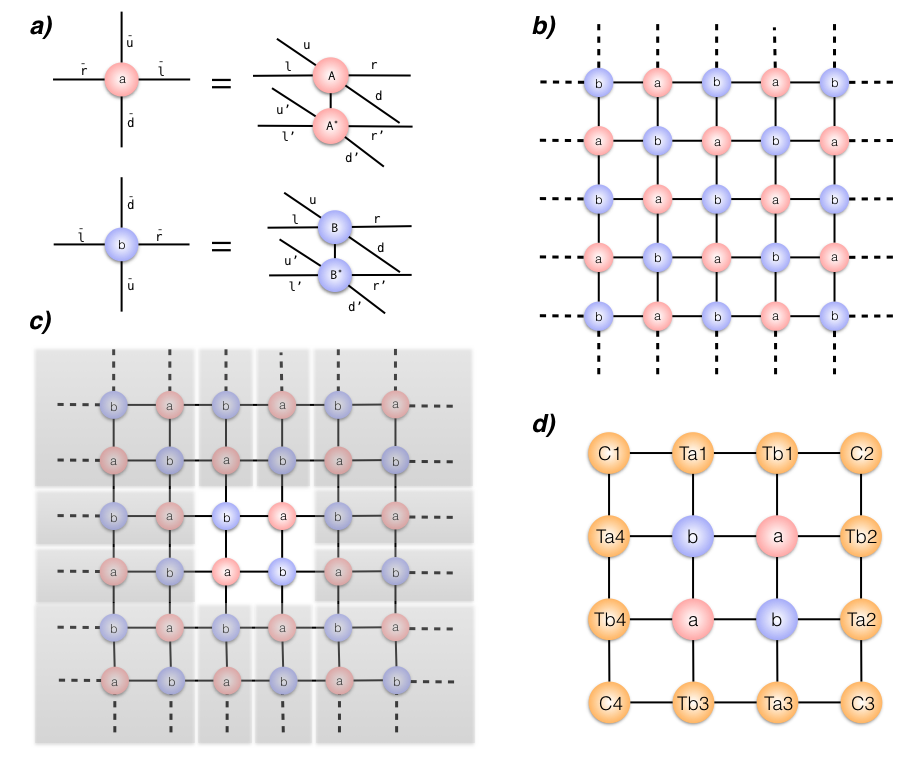
\includegraphics[width=0.75\textwidth]{figures/fig511.png}
	\caption[The picture of the main idea of itebd.]{The red and blue tensor denotes on \textit{odd} and \textit{even} sites. The yellow one are time evolution operators $e^{-\tau H_{k,k+1}}$, $e^{-\tau H_{k+1,k}}$}
	\label{fig511}
\end{figure}

For the approximation of environment, the directional variant of the CTMRG was developed. According to \textit{directional coarse-graining moves}, the effective environment could be updated from four different moves , left, right, up and down and iterated until the environments converges. 

For instance, the procedures to the left move, shown in the Fig. \ref{fig512} which is derived by Roman and Vidal, is made up of four major steps,
\begin{enumerate}
	\item Insertion: Insert two new columns which consist of \{ $T_{a1},b,a,T_{b3}$ \} and \{ $T_{b1},a,b,T_{a3}$ \} as in Fig. \ref{fig512}(b).
	\item Absorption: In order to obtaining two new corner matrices $\tilde{C_1}$ and $\tilde{C_4}$, and two new transfer matrices $\tilde{T_{b4}}$ and $\tilde{T_{a4}}$, we contract tensors $C_1$ and $T_{b1}$, tensors $C_3$ and $T_{a3}$, tensors $T_{a4}$ and $b$, and tensors $T_{b4}$ and $a$. Then, contract tensors $\tilde{C_1}$ and $\tilde{T_{b4}}$, and tensors $\tilde{C_4}$ and $\tilde{T_{a4}}$, obtaining $\tilde{Q_1}$ and $\tilde{Q_4}$ which play significant rules for calculating isometries between $\tilde{T_{b4}}$ and $\tilde{T_{a4}}$ as in Fig. \ref{fig512}(c).
	\item Renormalization: Truncate the vertical virtual bonds of $\widetilde{C_1}$, $\widetilde{T_{b4}}$, $\widetilde{T_{a4}}$, and $\widetilde{C_4}$ by contracting the isometries $Z$ and $W$, where
\begin{align}
	\label{isometry}
	&Z^{\dagger}Z = I \\
	&W^{\dagger}W = I
\end{align}
and the renormalization of the left CTM, yield as
\begin{align}
	\label{renormalize}
	&C^{\prime}_1 = Z^{\dagger} \tilde{C_1} \\
	&T_{b4}^{\prime} = Z\tilde{T_{b4}}W^{\dagger} \\
	&T_{a4}^{\prime} = W\tilde{T_{b4}}Z^{\dagger} \\
	&C^{\prime}_4 = Z\widetilde{C_4}
\end{align}
See the Fig. \ref{fig512}(d) and \ref{fig512}(f).
	\item Truncation: To determinate the isometries Z and W in the \textit{renormalization} steps is the most significant part. In this case, we use the eigenvalue decomposition of 
		\begin{align}
			\label{eigh_ctm}
			&\tilde{C_1}\tilde{C^{\dagger}_1}+\tilde{C_4}\tilde{C^{\dagger}_4}= \tilde{Z} D_z \tilde{Z^{\dagger}}\\
			&\tilde{Q_1}\tilde{Q^{\dagger}_1}+\tilde{Q_4}\tilde{Q^{\dagger}_4}= \tilde{W} D_w \tilde{W^{\dagger}}
		\end{align}
		shown in Fig. \ref{fig512}(e). It's not hard to find that the 
		the dimension of bonds of $D_z$ and $D_w$ increase to $\chi^2$. For that reason, we have to truncate $\tilde{Z}$ and $\tilde{W}$ to isometries $Z$ and $W$ which are equivalent to keeping the columns of $\tilde{Z}$ and $\tilde{W}$ corresponding to $\chi$ largest eigenvalues of $D_z$ and $D_w$.
\end{enumerate}

Now, we need repeat the procedures in Fig. \ref{fig512}(b)-(d) again for absorbing the other inserted column in Fig. \ref{fig512}(d) and obtain a new effective environment $G^{\prime \left[\vec{r_1},\vec{r_2},\vec{r_3},\vec{r_4}\right]}$ for the four-site unit cell. By composing four variant moves of the CTM we build an epoch of CTMRG. 

\begin{figure}[ht]
	\centering
	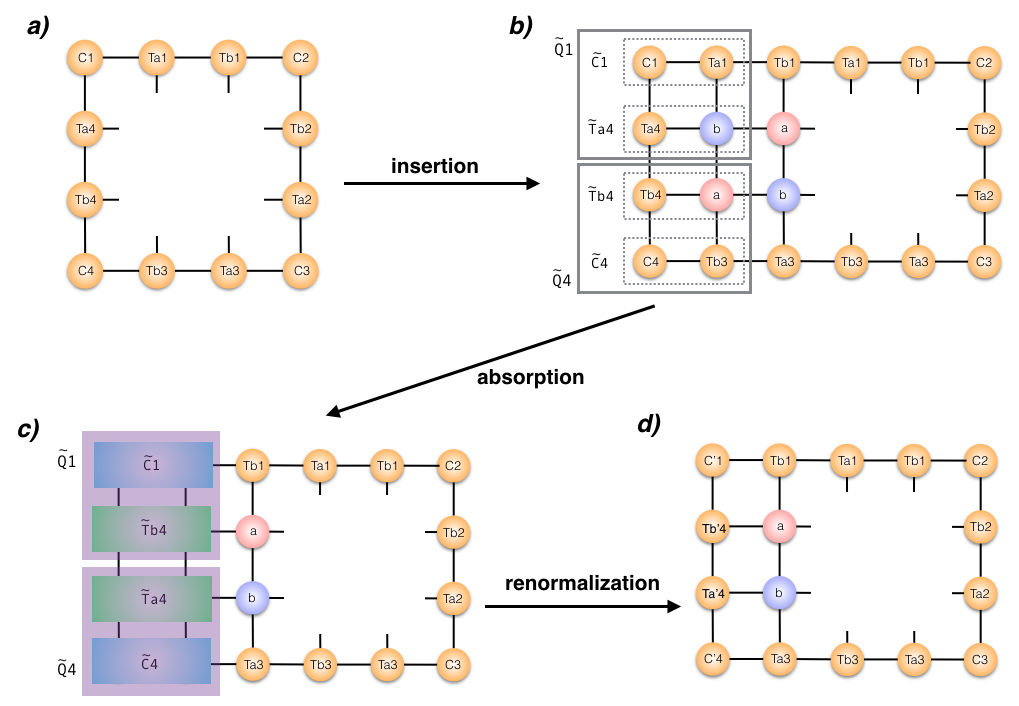
\includegraphics[width=0.80\textwidth]{figures/fig512.png}
	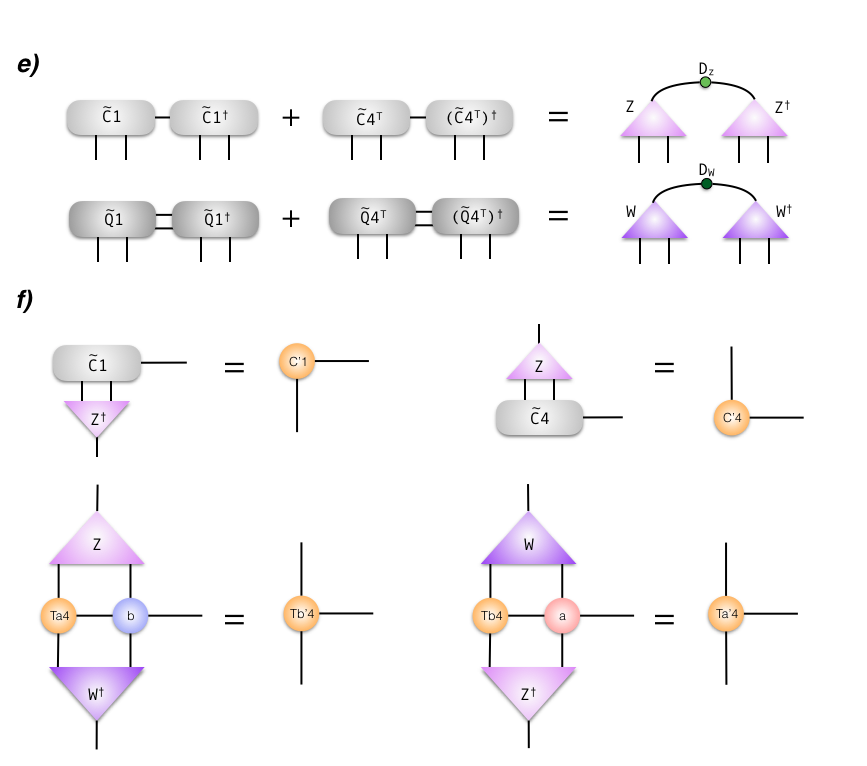
\includegraphics[width=0.80\textwidth]{figures/fig513.png}
	\caption[The picture of the main idea of itebd.]{The red and blue tensor denotes on \textit{odd} and \textit{even} sites. The yellow one are time evolution operators $e^{-\tau H_{k,k+1}}$, $e^{-\tau H_{k+1,k}}$}
	\label{fig512}
\end{figure}

\section{Obtain States from PESS}
\label{pessctm}
In this section, we apply the CTM to approximate the effective environment of 4-PESS structure. Firstly, we must transform it to iPEPS structure which is suit for the form of CTM. As shown in Fig. \ref{fig521}, the projection tensors, $U^{[0]}$, $U^{[1]}$, $U^{[2]}$ and $U^{[3]}$, and the entangled simplex tensors, $S^{[\alpha]}$ and $S^{[\beta]}$ are obtained from 4-PESS ansatz. To map these states to PEPS-like structure, we group the tensors, $S^{[\alpha]}$, $U^{[0]}$ and $U^{[1]}$, in red rectangles into the tensor $A$, 
\begin{align}
	A^{\sigma_i \sigma_j}_{i^{\prime}j^{\prime}kl} = \sum_{ij}{U^{[0]}_{ ii^{\prime},\sigma_i} S^{[\alpha]}_{ijkl} U^{[1]}_{ jj^{\prime},\sigma_j}}
\end{align}
and group, $S^{[\beta]}$, $U^{[2]}$ and $U^{[3]}$, in blue rectangles into the tensor $B$
\begin{align}
	B^{\sigma_k \sigma_l}_{i^{\prime}j^{\prime}kl} = \sum_{k^{\prime}l^{\prime}}{U^{[2]}_{ kk^{\prime},\sigma_i} S^{[\beta]}_{i^{\prime}j^{\prime}k^{\prime}l^{\prime}} U^{[3]}_{ ll^{\prime},\sigma_j}}
\end{align}
, whee the ranks of tensor $A$ and $B$ are six and there are two physical bonds contained in each of them. Hence, after combined the physical bonds in tensors $A$ and $B$, the iPEPS structure will be obtained,
\begin{align}
	A^{\sigma_i \sigma_j}_{i^{\prime}j^{\prime}kl} \rightarrow  A^{\sigma_A}_{i^{\prime}j^{\prime}kl} \\
	B^{\sigma_k \sigma_l}_{i^{\prime}j^{\prime}kl} \rightarrow  B^{\sigma_B}_{i^{\prime}j^{\prime}kl}
\end{align}
Next, in order to make the structure more balance, the entanglement should be well-distributed between each sites, 
\begin{align}
	\widetilde{A} = \sum_{i^{\prime}j^{\prime}kl}{\lambda^{[\beta]^{\frac{1}{2}}}_{i^{\prime}} \lambda^{[\beta]^{\frac{1}{2}}}_{j^{\prime}} A^{\sigma_A}_{i^{\prime}j^{\prime}kl}\lambda^{[\alpha]-\frac{1}{2}}_{l} \lambda^{[\alpha]^{-\frac{1}{2}}}_{k}}\\
	\widetilde{B} = \sum_{i^{\prime}j^{\prime}kl}{\lambda^{[\alpha]^{\frac{1}{2}}}_{k} \lambda^{[\alpha]^{\frac{1}{2}}}_{l} B^{\sigma_B}_{i^{\prime}j^{\prime}kl} \lambda^{[\beta]^{-\frac{1}{2}}}_{i} \lambda^{[\beta]^{-\frac{1}{2}}}_{j^{\prime}}}
\end{align}
and substitute $\widetilde{A}$ and $\widetilde{B}$ into Eq. \ref{reduce_a} and Eq. \ref{reduce_b} to obtain reduced tensors $a$ and $b$. In the end, we apply these two reduced tensor to build the form of CTM and follow the procedures shown in Fig. \ref{fig513} to simulate the effective environment tensors.

\begin{figure}[ht]
	\centering
	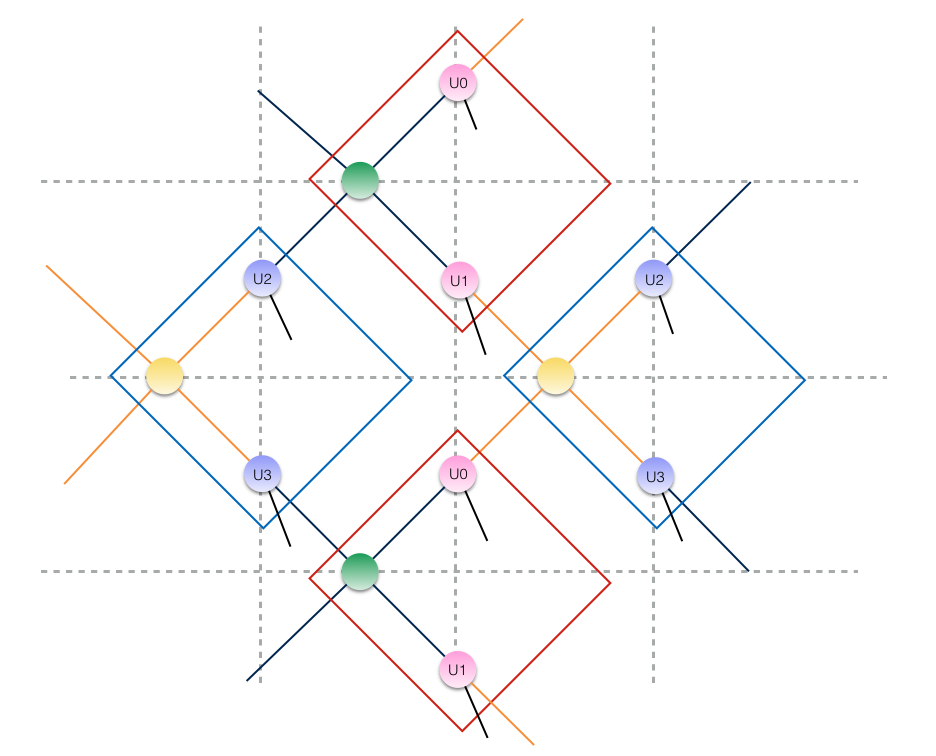
\includegraphics[width=0.80\textwidth]{figures/fig521.png}
	\caption[The picture of the main idea of itebd.]{The red and blue tensor denotes on \textit{odd} and \textit{even} sites. The yellow one are time evolution operators $e^{-\tau H_{k,k+1}}$, $e^{-\tau H_{k+1,k}}$}
	\label{fig521}
\end{figure}

\section{Comparison}

\begin{figure}[ht]
	\centering
	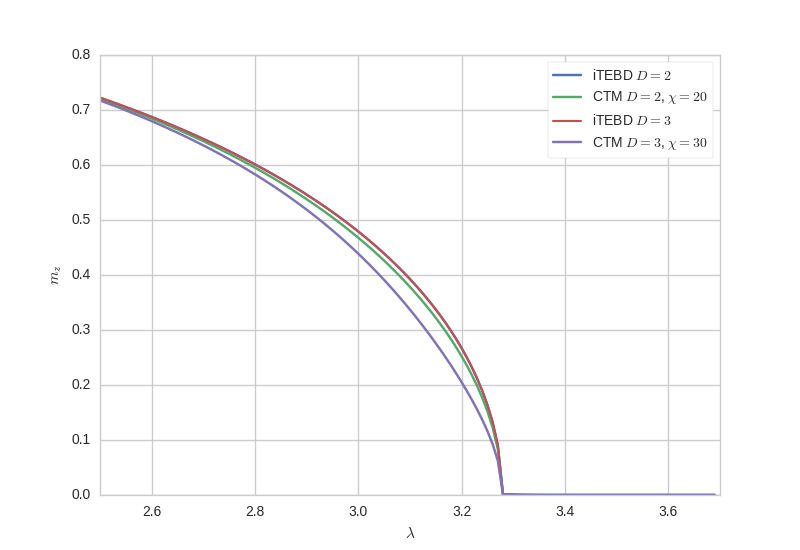
\includegraphics[width=0.80\textwidth]{figures/ctm_itebd.png}
	\caption[The picture of the main idea of itebd.]{The red and blue tensor denotes on \textit{odd} and \textit{even} sites. The yellow one are time evolution operators $e^{-\tau H_{k,k+1}}$, $e^{-\tau H_{k+1,k}}$}
	\label{fig522}
\end{figure}

\begin{figure}[ht]
	\centering
	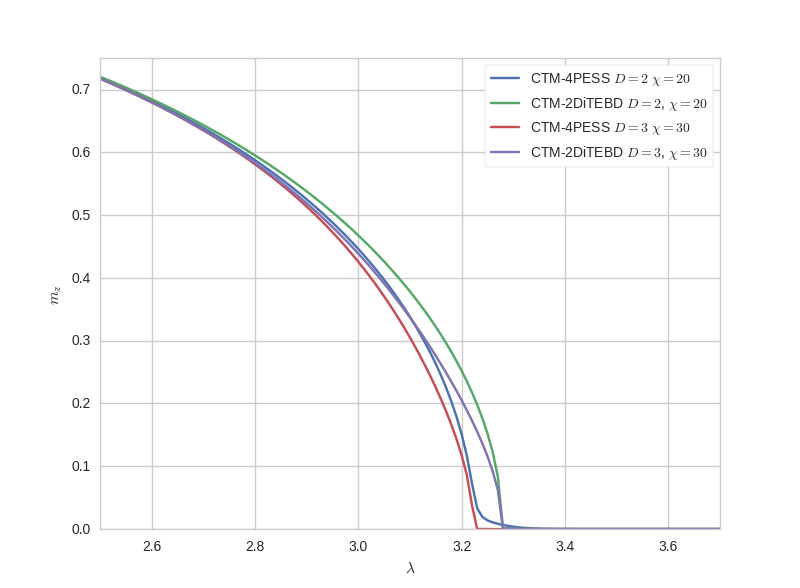
\includegraphics[width=0.80\textwidth]{figures/ctm_pess.png}
	\caption[The picture of the main idea of itebd.]{The red and blue tensor denotes on \textit{odd} and \textit{even} sites. The yellow one are time evolution operators $e^{-\tau H_{k,k+1}}$, $e^{-\tau H_{k+1,k}}$}
	\label{fig523}
\end{figure}


